\documentclass[a4paper,12pt]{article}

% For \url
\usepackage{hyperref}

% For line skip paragraphs
\usepackage[parfill]{parskip}

% For smaller margins
\usepackage[margin=1in]{geometry}

% For images
\usepackage{graphicx}
\usepackage{caption}
\usepackage{subcaption}

%For align environment
\usepackage{amsmath}

% For UTF-8
\usepackage[utf8]{inputenc}

% For verbatim environment
\usepackage{verbatim}

% Set section numbering to Roman
\renewcommand \thesection{\Roman{section}}
\renewcommand \thesubsection{\arabic{section}.\arabic{subsection}}

\title{TDT4258 \\ Energy Efficient Computer Design \\ Exercise 3}
\author{
    Lundal, Per Thomas \\ \texttt{perthol@stud.ntnu.no}
    \and
    Normann, Kristian \\ \texttt{krinorm@stud.ntnu.no}
    \and
    Selvik, Andreas Løve \\ \texttt{andrels@stud.ntnu.no}
}
\date{\today}

\begin{document}
\maketitle
\begin{abstract} % DONE!

This report presents a modular game engine implemented in C on the STK1000 development board running Linux. Furthermore we demonstrate the implementation of a game using said engine, and of drivers used by the engine to access the button and LEDs. This was done for exercise 3 in TDT4258, where we were asked to implement a game running on Linux which uses self-written drivers to interact with the peripherals.

\end{abstract}

\newpage
\tableofcontents

\clearpage
\section{Introduction} % DONE!

A major theme throughout computing history has been to set up appropriate levels for programmers to work in. These levels are typically related to how close to the hardware you need to be, depending on things like memory considerations and detailed hardware communication, ending up with a nice hierarchy from which developers can choose which level to do their work.

With reference to the two previous assignments, a great many details can be handled in low level programming. If you confine yourself to manipulating LEDs and mapping them to buttons, programming in assembly can be seen as appropriate. However, when the scope of the project is more complex, an alternative approach is required. In game development, splitting the code into multiple levels of abstraction, such as having hardware handling in low level and the handling of complex gameobjects in a higher, is usually prudent for any project of size. In such an event, using a high-level object-oriented programming language for the complex gameobjects will likely yield more readable, maintainable and effective code.

Visually, the final result of this project is a game similar to Space Invaders\cite{Space_invaders}, but that is of lesser importance and serves the role of that complex project. The assignment was to design and implement a game on the AVR32\cite{avr32} microcontroller using the sound, LED and button peripherals on the development board.  

In a sense, the levels in this project were \emph{drivers}, \emph{game engine} and \emph{game}. The driver level serves as the interface between hardware and software by setting up devices and enabling them for use. The game engine will then implement game-specific functions for them as well as creating an environment for easy game development. Finally, the game will make use of the game engine.

\clearpage
\section{Description And Methodology}

\subsection{Jumper and cable configuration} % DONE!
The jumpers were set as specified in the compendium\cite{compendium}

\begin{itemize}
\item The LEDs were connected to PIOB by a flat-cable from GPIO pins 8-15 to the LED pins on the STK1000. 
\item The buttons were connected to PIOB by a flat-cable from GPIO pins 0-7 to the LED pins on the STK1000.
\end{itemize}

\subsection{Linux} % DONE!

We started by following the guidelines and using the files posted on It’s Learning. We flashed the STK1000 with the bootloader U-Boot using the JTAGICE, and followed the steps to create a bootable SD card and copy the Linux system files and kernel to it. Except for a minor hassle when partitioning the SD card, everything went smooth.

We then connected the STK1000 to the computer via serial cable (RS-232), and started Minicom with the command “minicom -D /dev/ttyS0”. The guide stated; “Hardware Flow Control” should be disabled from the menu within Minicom, we accomplished this after searching through several submenus to find it.

Once we rebooted the board, lines of text began appearing in Minicom, proving that it was set up correctly. However, the joy of success quickly dissipated as we were met by the error message “ERROR: Can’t get kernel image”.

We decided the best action would be to try the files found on the external website. We flashed the SD card with the pre-made image using \emph{dd}, and flashed the new version of U-Boot. This however, did not yield any progress as we were met with the error message “No MMC card found” in addition to the previous one.

After some back and forth between different versions we discovered that the boot command was incorrect, as it said to look for the kernel in the “/” folder instead of the “/boot” folder on the SD card. Fixing this allowed us to progress in the boot process, as it managed to load the kernel. However, the joy was once again short-lived as it gave us the error message “Unknown Architecture (0x11)” when trying to boot the kernel.

After more web searches we discovered that the Unknown Architecture error was caused by an obsolete U-Boot version made before AVR32 was granted its architecture number of 0x11. By combining the U-Boot from the external webpage with the slightly modified boot commands from the It's Learning version, we were finally able to boot the kernel.

There was, however, one final issue as the kernel failed to mount the SD card to load files. This was fixed by changing “rootwait=1” to “rootwait” in the boot arguments. We were now finally able to log into and start using our linux installation. To make sure we could reboot easily, we saved the boot commands and arguments with \emph{saveenv} in U-Boot.

\subsection{Hardware}

\subsubsection{Linux drivers} % DONE!

The purpose of the drivers is to function as the kernel-hardware interface. It is the driver's job to initialize the hardware and connect to the kernel, and specifically in the case of the linux kernel, to implement the functions $\_\_init driver\_init$ and $\_\_exit driver\_exit$ to communicate with the kernel. This implies setting up the driver and adding it to the system. Consecutively, additional driver-specific functions are implemented to handle the hardware.

\subsubsection{LEDs and buttons} % DÆNN!

As in the previous assignments, handling the LEDs starts by initializing the hardware.

\begin{verbatim}
	piob_pins = 1000000000000011110011100000000
	AVR32_PIOB.per = piob_pins;
	AVR32_PIOB.oer = piob_pins;
	AVR32_PIOB.codr = piob_pins;
\end{verbatim}

where $piob\_pins$ denote (as one might suspect) the pins for the LEDs. The reason for using strangely numbered pins of PIOB instead of the first 8 of PIOC is that PIOC is used for the ethernet port, and writing data to it will make the driver crash (we learned this the hard way).

The buttons are initialized similarly.

\begin{verbatim}
	piob_pins = 000000000000000000000011111111
	AVR32_PIOB.per = piob_pins;
	AVR32_PIOB.puer = piob_pins;
\end{verbatim}

In the LED driver, we use a characters to represent our LEDs (A-H), where an uppercase letter designates that a led is lit and a lowercase letter designates that it is unlit. The $driver\_read$ function works by iterating through all the pins, checking if the LED is lit or unlit, and returning the appropriate character. The $driver\_write$ function parses each character it receives to determine what pin to update.

We implemented the button driver analogously to begin with, but later changed it due to better compliance with our game engine. Now, $driver\_read$ works by reading the bits of each individual pin and returning a byte consisting of the state of all 8 pins. This is implemented by inverting the \emph{pdsr} and masking out the last 8 bits.

\subsubsection{Sound} % DONE!

At first we were confused by the fact that writing to the sound device \emph{/dev/dsp} as specified in the compendium \cite[p.60]{compendium} did not produce any sound. Neither did any other devices in \emph{/dev} that sounded like they could produce sound. However, we were relieved to discover that it was due to the volume being muted by default in \emph{Alsamixer}, and not a hardware or software issue.

Once we were able to produce sound, we decided to test our MIDI player. For an in-depth description of its inner workings, see Exercise 2 \cite{ex2}. Since we had portability in mind when creating the MIDI player, the only piece of code needed to be changed was the sample rate, in addition to scaling the output down from 16-bit to 8-bit to match the default values of the sound driver. However, this did not produce nearly as clean sound as expected.

We therefore looked into the \emph{ioctl} command, as suggested by the compendium \cite[p.60]{compendium}, which is used to pass settings to the driver. By setting the \emph{SOUND\_PCM\_WRITE\_RATE} and \emph{SOUND\_PCM\_WRITE\_BITS} values we increased the sample rate to 22 KHz and bit depth to 16 bits, which resulted in crystal clear sound once again.

\subsubsection{Screen} % DONE!

In spirit of real engineering we started by writing random data to \emph{/dev/fb0} to see the result. Once we knew that it was a simple matter of dumping data to the file, we set out to create a program to display basic colors and shapes.

We started by opening the file. The description of the screen pixel data in the compendium \cite[p.60]{compendium} stated that the screen used 32 BPP (Bits Per Pixel) where the first three bytes would read as the blue, green, and red values and the last byte would remain unused. With this in mind, we repeatedly wrote the values “0xFF 0xFF 0xFF 0x00” in hope of the pixels turning white, albeit, they did not. While some did, black lines were prevalent. After experimentation with different values, we discovered that the screen did in fact use a 24 BPP with no unused byte, explaining our troubles.

Now that we were able to fill the screen with simple colors, we began to create our graphics library. We started by implementing memory mapping, as it allows for individual pixels to be modified more easily, and by recommendation in the compendium \cite[p.60]{compendium}. We further implemented functions for filling the whole screen with a color and for drawing a rectangle with a color, this was done by looping through the pixels and setting the correct color data.

After having tested and verified that the rectangles were produced correctly, we decided to implement a very simple version of the game “Pong” to test the system\footnote{The controls does no longer work as intended due to a change in the button driver.}. This was accomplished by using 3 white rectangles; one for each paddle and one for the ball. The two paddles were set to move on button input, and the ball set to always move diagonally and reverse X or Y direction on collision with the top and bottom edges or a paddle. If it made it's way past a paddle to the left or right edges, it was simply moved to the middle and direction reversed. A screenshot can be seen in figure \ref{fig:pong}.
 
\begin{figure}
\centering
\fbox{\includegraphics[width=0.5\textwidth]{pong}}
\caption{Simple Pong implementation }
\label{fig:pong}
\end{figure}

We noticed quite a lot of flickering, because all objects were removed by painting over with a black rectangle and then drawn at their new position for each step. To combat this, we implemented \emph{double buffering} which means that we render the scene completely in an internal buffer before sending it to the screen. This reduced the performance though, as all pixels had to be copied from the buffer to the screen. However, this was compensated by implementing a function to only update a small rectangle of the screen. In addition, we found that replacing the for-loop that copied data to the screen with memcpy improved speed.

To prevent segfaults and wrapping to the next line (because the screen is a one-dimensional array of pixels) when specifying coordinates outside the screen we had to add some calculations to crop the end coordinates. This was accomplished by using some simple minimum and maximum operations.

\subsubsection{BMP} % DONE!

While rectangles are fine, they are not the same as images. Since we wanted to sprites and other images for our game, we looked into different image formats. BMP was by far the least complex, as it is only header data followed by raw pixel data \footnote{BMP supports a wide variety of different color formats, including color palettes, but we will only be using and supporting 24 BPP with 8 bits per color for simplicity.}. Work began by using the spesification found on wikipedia \cite{BMP_file_format} in combination with a simple implementation found on stack overflow \cite{stackoverflow_bmp}.

At first we had problem getting the correct data from the headers. Among other things it would return a negative value for file size. By printing byte data we found the problem to be that BMP uses little endian while AVR32 uses big endian, which forced us to reverse the order of the bytes in all the attributes of the headers. Afterwards, it was a simple matter of copying the raw pixel data and image dimensions to a struct. However, since BMP pads the width to a multiple of 4 bytes, we had to make it skip the excess data. A thing to note is that BMPs store the image from the bottom up, the opposite of normal conventions. This somewhat complicated the drawing methods and especially the screen edge cropping.

Since we wanted to have transparency but did not want to include an alpha channel as it would require costly multiplications for every sub-pixel upon drawing, we referred to the standard convention of using \emph{magic pink} where the color fuschia (\#FF00FF) is treated as transparency. This leaves jagged edges as there is no partial transparency, but is faster and therefore suits our purpose better. In addition, we made a tint function so that we could create generic images and then tint them on the fly to suit our needs (this became useful for power-ups and text).

\subsubsection{Text} % DONE!

We wanted to be able to print any text string to the screen without creating individual images for each of them, and therefore needed some kind of font system. We looked online for a good font that could easily split to individual BMP files. We decided to use Visitor \cite{font}, as it had two sizes, looked good, and had hard edges (no semi-transparent pixels). After slightly modifying the large version to make it less pixelated, each character was put into its own image and saved as a BMP file where the name was that character’s hexadecimal ASCII character code \cite{ascii}, splitting the different fonts into different folders.

This allowed us to choose a font by specifying a folder, and simply convert each character in the text to hexadecimal to find the corresponding image that should be drawn on the screen. Additionally, we added support for setting the character spacing, background color, and background margins.

\subsection{Game Design} % DONE!

To make this exercise as modular as possible, we decided to make a general game engine before we actually went about making a game. We decided on making a game where we'd be able to add game-objects (visual things in the game, nouns) to the game and subsequently add ‘components’ to them. That is, behaviours (verbs) such as a death function, collision behaviour, etc.

\subsubsection{Game Engine} % DONE!

\begin{figure}[h]
\centering
\begin{verbatim}
    while (ENGINE_RUNNING) {
         engine_tick();
         engine_draw();
         TICK++;
     }
\end{verbatim}
\caption{The essential part of the main loop in the game engine}
\label{fig:mainloop}
\end{figure}

The core of the game engine is its tight update loop, see figure \ref{fig:mainloop}. \emph{engine\_tick()} steps the game logic by one tick and produces an array of drawable objects that constitutes the current frame. \emph{engine\_draw()} draws the resulting frame to the screen. As seen from figure \ref{fig:mainloop} these two functions are executed repeatedly after one another as long as the engine runs. Note that there is a parallelization potential here.

The game logic in the engine is structured as a game where \emph{engine\_tick()} is a traversal of said tree, calling a tick function at each node. There is an array of function pointers to \emph{ticker\_functions} that \emph{engine\_tick()} iterates over, calling every function pointed to. These functions can then iterate through and call functions of their own, creating the tree structure. The general structure can be seen in figure \ref{fig:enginecore}.

\begin{figure}
\centering
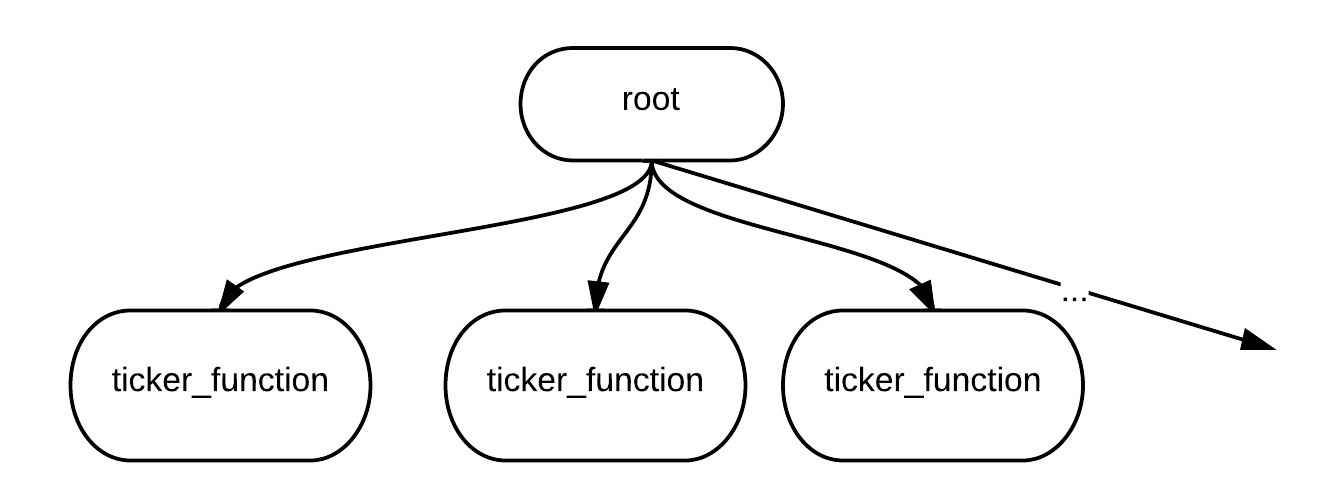
\includegraphics[width=0.5\textwidth]{general_engine}
\caption{The core update loop of the engine}
\label{fig:enginecore}
\end{figure}

One particular \emph{ticker\_function} that is central to the game engine is the \emph{gameobject\_ticker}, which is responsible for the logic and draw queuing of all the objects in the game. Every object in the game corresponds to an instance of the \emph{gameobject} struct, see figure \ref{fig:gameobjectdef}. But, the \emph{gameobject} struct itself only contains minimal information, such as position and health, so almost all of the functionality comes from the components stored in its array called \emph{components}. A \emph{component} is a struct with three function pointers, see figure \ref{fig:component}, \emph{add\_function} is called once when the component is added to a gameobject and \emph{remove\_function} when the component is removed. As long as the component is part of an active gameobject’s list of components, its \emph{tick\_function} will be called every game tick. This structure makes a tree, see figure \ref{fig:gameobjecttree} which serves as a subtree of the overall update tree.

\begin{figure}[h]
\centering
\begin{verbatim}
typedef struct {
    component **components;
    void **components_data;
    int pos_x;
    int pos_y;
    int size_x;
    int size_y;
    int hp;
    int type;
 } gameobject;
\end{verbatim}
\caption{Essential parts of the gameobject struct}
\label{fig:gameobjectdef}
\end{figure}

\begin{figure}[h]
\centering
\begin{verbatim}
// Define function pointer 
typedef void (*component_function)(int component_nr, gameobject *object, void *param); 
  
// Components consists of three functions 
typedef struct { 
    component_function add_function; 
    component_function tick_function; 
    component_function remove_function; 
} component;

\end{verbatim}
\caption{The component struct definition}
\label{fig:component}
\end{figure}

\begin{figure}
\centering
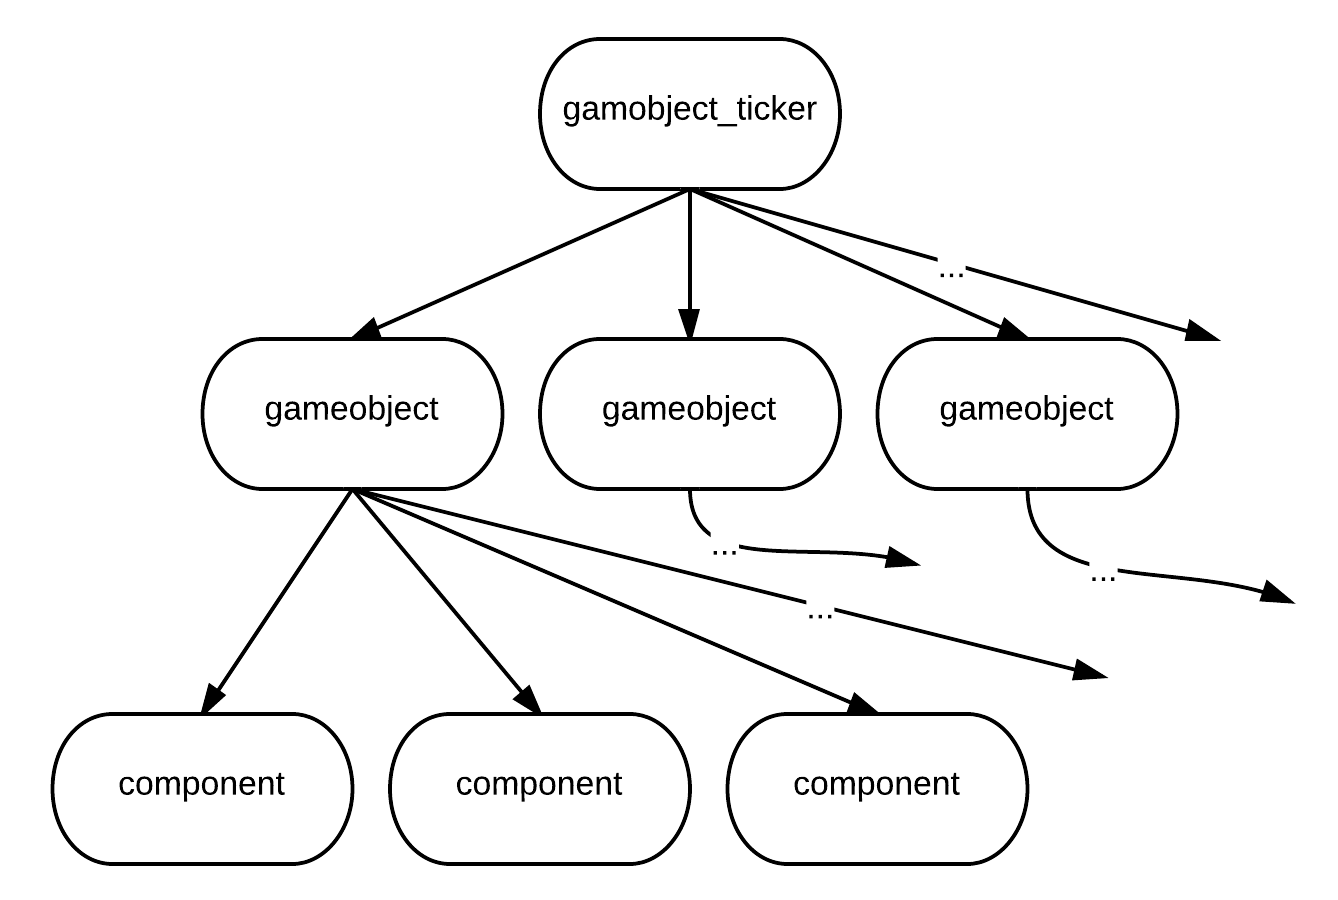
\includegraphics[width=0.6\textwidth]{gameobject_ticker}
\caption{The general gameobject architecture}
\label{fig:gameobjecttree}
\end{figure}

As a concrete example of how a tree might look in a game, see figure \ref{fig:enginesnapshot} which is a snapshot of how the game tree might look at some point in time in our engine. This tree will be traversed every tick, calling functions of nodes, which is where all the game logic in our game happens.

\begin{figure}
\centering
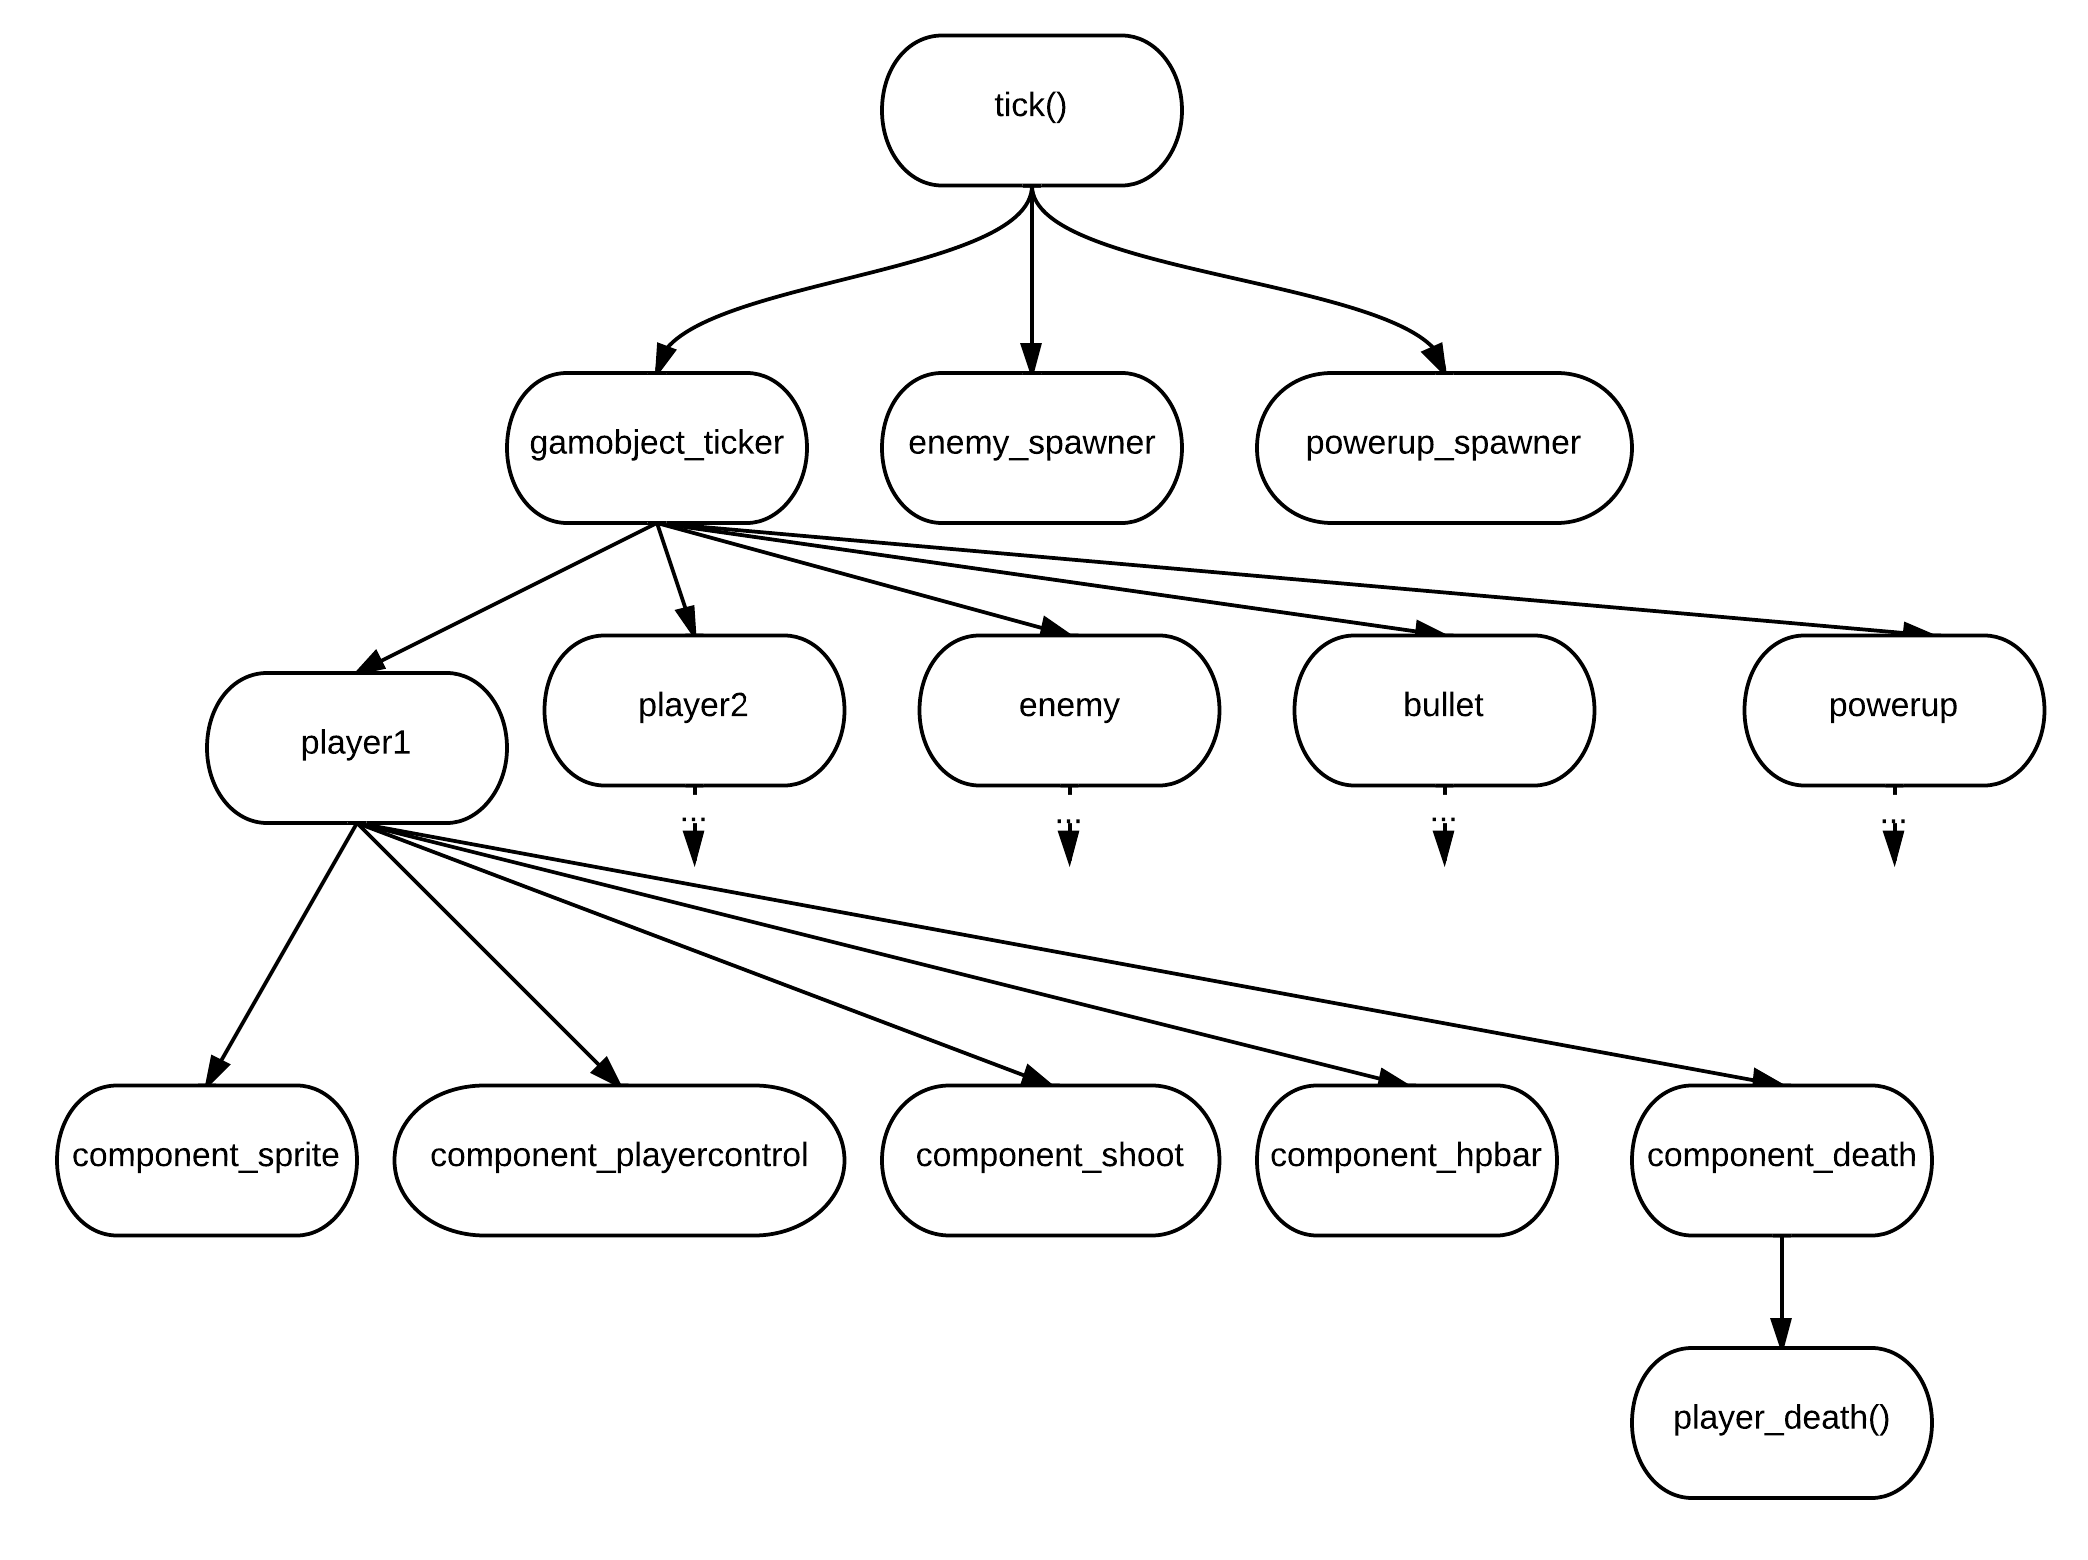
\includegraphics[width=\textwidth]{gametreesnapshot}
\caption{The gametree from a snapshot of our game}
\label{fig:enginesnapshot}
\end{figure}

In order for components to be able to store data between calls we gave the gameobjects an additional array of void pointers called \emph{components\_data}, see figure \ref{fig:gameobjectdef}, where each component can store whatever they want. That is, the component stored in \emph{components[i]} can use the void pointer in \emph{components\_data[i]} for storing any data. This way, components can also access and edit the data of other components as long as it knows what number the component has and how it stores its data. 

This modular component based game architecture gives a lot of flexibility as components and game objects can be added, removed and modified at any time. It can also be combined in any way desirable. Say you want to make a player mind control an enemy; just add a \emph{player\_control} component to it, and it will work right away.

\subsubsection{Noteworthy components} % DONE!

\textbf{\emph{component\_sprite:}} This component adds a \emph{drawable} to the draw queue at the position of the calling \emph{gameobject} every tick. In our game this is the only component that adds to the draw queue and is therefore responsible every image visible on the screen.

\textbf{\emph{component\_death:}} Takes a function pointer as an argument and executes said function when the game object’s hp falls to or below 0. It then removes itself, so the function is only called once. We use this component in our game to make power-ups spawn when enemies die and to end the game when a player dies.

\textbf{\emph{component\_collision:}} Scans all game objects and checks if it collides with any of a given type. If so, it will add a component to it and one to itself. Pointers to these components are taken as an argument to this component, making this a very flexible component that can incorporate a wide spectre of different behaviours. We use this component in our game to make bullets deal damage to their targets and make the power-ups add a powerup component to the player, etc.

\textbf{\emph{component\_powerup:}} This component lights up a given LED, and when the button matching the LED is pressed adds a given component to the player firing it and one to the other player. In combination with \emph{component\_collision}, this is used to make the power-up orbs work the way they do.

\subsubsection{The Game} % DONE!

The game is a 2-player 2D game in which each player commands a rabbit. The task is to survive hordes of attacking UFOs while trying to take each other out. If one player dies the other is victorious. If both die (at the same time), both lose.

Both rabbits have 32 hp (hitpoints) and lose hp if a ufo passes by them. If a rabbit is hit by a ufo, that rabbit loses hp and the ufo is destroyed. There are also some power-ups that occasionally appear on the screen. If a rabbit gets a power-up, the LED corresponding to that power-up lights up, meaning that the rabbit now has a round of that power-up in its arsenal.

The rabbits only move horizontally on the screen. Player 1 uses buttons SW0 and SW1 for power-ups and SW2 and SW3 for movement, while player 2 uses buttons SW7 and SW6 for power-ups and SW5 and SW4 for movement.

There are three types of power-ups:
\begin{itemize}
\item \emph{Swap-health:} The rabbit swaps hitpoints with the other rabbit
\item \emph{Mind-control:} Gives the commanding rabbit a tiny heal and mind controls the other rabbit to move as you do for a short while.
\item \emph{Healing:} Instant heal.  
\end{itemize}

\begin{figure}
\centering
\fbox{\includegraphics[width=0.5\textwidth]{screenshot}}
\caption{The game in action}
\label{fig:game}
\end{figure}

\subsection{Tools} % DONE!

\begin{itemize}
\item GitHub for handling version control
\item Vim as main code-editor
\item Google Docs for report collaboration
\item \LaTeX for report markup
\item \url{https://www.lucidchart.com/} in order to make the diagrams
\item \url{https://www.writelatex.com/} for writing
\item Our self written ip.c which shows the current ip on the screen. This was run on boot such that we could ssh into the board without having to go through minicom first.
\end{itemize}

\clearpage
\section{Results And Tests}
To test our graphics library, we wrote a program testing it where we made sure to include the edge cases. See test 1 and 2 in the appendix.  A couple of pictures are drawn where some of them are tinted and some of them are partly outside the screen. The result is shown in figure \ref{fig:tint_and_edge}, which clearly indicates that it works as intended. 

Test 3 and 4 were designed and used to test our drivers, and they both work. Test 4 works because the buttons pushes a byte with bits set in the same way the buttons are held down. This way we can encode ascii bytes by pushing the correct binary number on the buttons. This did indeed work.

To stress test our game engine, we wrote a benchmark game which spawned a lot of game objects and recorded the frame rate with different amounts of objects. This was rerun with different components in the objects. See figure \ref{fig:sprite_graph} and \ref{fig:sprites_collision_bg_graph}. 

\begin{figure}
\centering
\includegraphics[width=0.8\textwidth]{tint_and_edge-test}
\caption{The test for tinting and no-edge-wrapping for pictures}
\label{fig:tint_and_edge}
\end{figure}

\begin{figure}
\centering
\includegraphics[width=0.8\textwidth]{sprite_graph_2}
\caption{The framedrop as gameobjects with only a sprite component are added}
\label{fig:sprite_graph}
\end{figure}

\begin{figure}
\centering
\includegraphics[width=0.8\textwidth]{sprites_collision_bg_graph_2}
\caption{The framedrop as gameobjects with a sprite component and a collision component are added}
\label{fig:sprites_collision_bg_graph}
\end{figure}

\clearpage
\section{Discussion}

The most obvious thing we can see from the stress test is that drawing the background image has a significant, but constant, effect on the frame rate.

Further, we can see that even though the collision component does a search through every other game object every tick, which is an $O(n^2)$ operation, but it does not seem to have such a significant impact on the fps. This might be because there is only a single comparison done within the loop and iterations in C are efficient, but it also shows that the main bottleneck seems to be the drawing. 

Lastly, it is worth noting that throughout the development of the actual game on our engine, we experienced virtually no segfaults or bugs. As students without too much earlier experience in C this is rare, and we noticed that other groups had more trouble. This is either a lot of luck, or a sign that our game engine is pretty stable.


\subsection{Further work}

A game engine is a big and complex beast, and as such there are many improvements that could be made in the future. Here are some pointers to areas that might be the focus of future work.

The definition of the game, that is, the setup of initial game object and their components are done in a .c file. As games gets bigger, this will be a significant amount of code, or rather data. The problem here is that we put data straight into code, meaning that if you were to tweak anything in the game, you need to recompile. Splitting the data from the code would involve writing a parser of game data from some file format, say xml. This is some work, but make a significant impact on the usability of the engine for bigger games.

The draw function and the traversal of the game tree are only coupled via the draw queue. There is an opportunity for running these function in two different threads. While this will introduce some more complexity in the form of concurrency issues, some of which might be solved by introduction two instances of the draw queue and swapping before each game tree traversal, there could be a significant performance gain. The performance gain is dependent on the processor architecture; the avr32 processor is not multi-core, but if it is superscalar, there might still be an improvement.

Yet another feature which could be implemented which might be required for more advanced games is some sort of draw layers. This can be implemented by either making the draw queue a two-dimensional array instead of one-dimensional, where the second dimension would be the layer, and draw the layers sequentially, or by passing a z value with each drawable and then sort the array on that value before drawing.

As the framerate is not constant, one should look into doing the game logic on the time since last tick instead of using ticks directly. This will the game happen at a constant real time speed. This will however, unless one takes care to work in ms, include floating point operations which might reduce the performance of the engine.

\clearpage
\section{Evaluation Of Assignment}

The compendium and recitation slides states that the screen is using 32 bpp. It is in fact using 24 bpp; 8 bits per color.

Had some trouble to get sound to work because we did not realize the output was muted. This was explained in the guide, but we nearly abandoned that as it mostly gave us trouble in the beginning.

\clearpage
\section{Conclusion}

We have created a modular and powerful game engine running our rabbit game on the STK1000. As seen in the results, the game engine can handle a big number of game objects before dropping to unplayable frame rates. The engine makes use of our linux drivers to access the button and LED peripherals.

\clearpage
\begin{thebibliography}{9}

\bibitem{ex2}
P.T. Lundal, K. Normann and A.L. Selvik,\\
\emph{TDT4258 Energy Efficient Computer Design Exercise 2},\\
2013.

\bibitem{compendium}
Computer Architecture And Design Group, \\
\emph{Lab Assignments In TDT4258 Energy Efficient Computer Systems}.\\
Department Of Computer And Information Science, NTNU, 2013,\\
\url{http://www.idi.ntnu.no/emner/tdt4258/_media/kompendium.pdf}

\bibitem{avr32}
Atmel, \\
\emph{AVR32 Architecture Document},\\
2011,\\
\url{http://www.idi.ntnu.no/emner/tdt4258/_media/doc32000.pdf}

\bibitem{ap7000}
Atmel,\\
\emph{AT32AP7000 Preliminary},\\
2009,\\
\url{http://www.idi.ntnu.no/emner/tdt4258/_media/doc32003.pdf}

\bibitem{Space_invaders}
\emph{Space Invaders},\\
Wikipedia, 2013,\\
\url{http://en.wikipedia.org/wiki/Space_Invaders}

\bibitem{BMP_file_format}
\emph{BMP file format},\\
Wikipedia, 2013,\\
\url{http://en.wikipedia.org/wiki/BMP_file_format}

\bibitem{stackoverflow_bmp}
\emph{read bitmap file into structure},\\
Stack Overflow, 2013,\\
\url{http://stackoverflow.com/questions/14279242/read-bitmap-file-into-structure}

\bibitem{font}
Ænigma,\\
\emph{Visitor},\\
Dafont, 2013,\\
\url{http://www.dafont.com/bitmap.php}

\bibitem{ascii}
\emph{ASCII Table and Description},\\
AsciiTable, 2013,\\
\url{http://www.asciitable.com/}

\end{thebibliography}

\clearpage
\appendix
\addcontentsline{toc}{section}{Appendix}
\section{Tests}

\begin{tabular}[h]{|lp{12cm}|} \hline
\textbf{\emph{Test 1:}} 	& \textbf{Tint test}\\
\emph{Action:} 		& Load an image. Tint it. display it.\\
\emph{Wanted outcome:}	& It has been drawn with the colour we tried to paint it with \\ \hline
\end{tabular}
\vspace{1cm}

\begin{tabular}[h]{|lp{12cm}|} \hline
\textbf{\emph{Test 2:}} 	& \textbf{Screen edge test}\\
\emph{Action:} 		& Draw a picture on the screen such that it extends outside.\\
\emph{Wanted outcome:}	& 1) No crash. 2) Picture doesn’t wrap to next line. \\ \hline
\end{tabular}
\vspace{1cm}

\begin{tabular}[h]{|lp{12cm}|} \hline
\textbf{\emph{Test 3:}} 	& \textbf{LED driver test}\\
\emph{Action:} 		& Write the data AbCdEfGh to emph{/dev/leds} \\
\emph{Preconditions:}	& LED driver loaded.\\
\emph{Wanted outcome:}	& Even numbered LEDs should turn on and odd numbered LEDs should turn off \\ \hline
\end{tabular}
\vspace{1cm}

\begin{tabular}[h]{|lp{12cm}|} \hline
\textbf{\emph{Test 4:}} 	& \textbf{Button and LED driver test}\\
\emph{Action:} 		& 1) \emph{cat} button output to leds. 2) Test pushing ASCII combinations.\\
\emph{Preconditions:}	& Button and LED driver loaded.\\
\emph{Wanted outcome:}	& LED 0..7 should turn on for values 65..72 and off for values 97..104.\\ \hline
\end{tabular}
\vspace{1cm}

\begin{tabular}[h]{|lp{12cm}|} \hline
\textbf{\emph{Test 5:}} 	& \textbf{Frames-Per-Seconds(FPS) and gameobjects}\\
\emph{Action:} 		& Start the game and, at certain time intervals, add 50 enemy gameobjects, and write out the FPS as the number of gameobjects on the screen increases.\\
\emph{Expected outcome}	& A gradual drop in FPS towards.  \\ \hline
\end{tabular}
\vspace{1cm}

\end{document}

